% =====================================================================================
% Replanning Against a Saboteur -- IEEE conference format (IEEEtran).
% Course requirements: Times New Roman 12 pt, 1.25 line spacing, at least 10.5 pages.
% Compiles on Overleaf with pdfLaTeX (Menu -> Compiler: pdfLaTeX) + BibTeX.
% All numbers in tables come from paper/make_tables.py (generated from results/*.csv);
% all numbers in the text are copied from results/SUMMARY.md.
% =====================================================================================
\documentclass[conference,12pt]{IEEEtran}

\usepackage[T1]{fontenc}
\usepackage{amsmath}
\usepackage{newtxtext,newtxmath}   % Times New Roman text and maths
\usepackage{setspace}
\setstretch{1.25}                  % course requirement: 1.25 line spacing
\usepackage{graphicx}
\usepackage{booktabs}
\usepackage{cite}
\usepackage{url}
\usepackage{algorithm}
\usepackage{algpseudocode}
\usepackage{xcolor}
\graphicspath{{figures/}}
\newcommand{\dstar}{D*~Lite}

\begin{document}

\title{Replanning Against a Saboteur: Does Incremental Search Still Save Effort When the Opponent Blocks the Route?}

% STUDENT: replace with your group's names, roll numbers and affiliation.
\author{\IEEEauthorblockN{Author One, Author Two, Author Three, Author Four}
\IEEEauthorblockA{Fundamentals of Artificial Intelligence, Section ??, Group ??\\
Department ??, University ??\\
Email: ??}}

\maketitle

% STUDENT REVIEWS: check every sentence and number of the abstract against results/SUMMARY.md.
\begin{abstract}
Game characters that walk through a changing world must replan, and incremental
search algorithms such as \dstar{} promise to do so more cheaply than searching again from
scratch. Most evaluations change the map at random. We ask what happens when the opponent
changes it on purpose: a \emph{saboteur} that blocks the cell on the character's planned path
that lengthens its trip the most. We port the search code of our grid game, \emph{Outwit}, to
Python, verify it against the game's own test numbers, and compare BFS and A* that replan from
scratch, a \emph{lazy} A* that replans only when its path is broken, and \dstar{}, on 360
problems from 24 real game maps of the Moving AI benchmarks (5760 runs). Four findings emerge.
(1)~Against random blocks, lazy A* has the lowest total search effort: \dstar{}'s first plan
costs a median 1.84$\times$ A*'s, and the few replans that random blocks cause never pay this
back. (2)~Against the saboteur, \dstar{} needs about 4$\times$ fewer expansions than both A*
variants (86{,}989 vs.\ 354{,}770 on average; fewer in 305 of 360 problems), because every
saboteur block hits the planned path and forces lazy A* to replan every time. (3)~The worst
single replan, the ``hitch'' a player would notice, is not reliably reduced: the paired test
favours \dstar{} only weakly overall (Holm $p=0.042$) and not at all on two of the three map
sets. (4)~In our Python implementation, a \dstar{} expansion costs 3--4$\times$ as long as an A*
expansion, which cancels its expansion savings in wall-clock time.
\end{abstract}

\begin{IEEEkeywords}
heuristic search, incremental search, D* Lite, A*, replanning, game AI, network interdiction
\end{IEEEkeywords}

% =====================================================================================
\section{Introduction}
% =====================================================================================

A non-player character (NPC) in a video game often has to walk from one place to another while
the world changes around it: doors close, crates fall, and, in many games, the player
deliberately puts obstacles in its way. Each change can make the character's current route
invalid or suboptimal, and the character must then \emph{replan}. Game AI usually does so in
the simplest way, by running A*~\cite{hart1968astar} again from the character's current
position~\cite{orkin2006fear,uludagli2023npc}. Incremental heuristic search
algorithms~\cite{koenig2004incremental} such as Focussed D*~\cite{stentz1995focussed},
Lifelong Planning A*~\cite{koenig2004lpa} and \dstar{}~\cite{koenig2002dstarlite,koenig2005fast}
were designed for this situation: they keep the results of the previous search and repair
only the part that the change has made wrong. For robots that discover obstacles gradually,
they are known to save a large amount of work~\cite{koenig2005fast}.

Whether they also save work in a game is less clear. Hern{\'a}ndez et
al.~\cite{hernandez2012poorly} pointed out that it is not well understood when \dstar{} is
actually faster than repeated A*, and later showed that a carefully designed A* variant can
beat it on common map types~\cite{hernandez2014mpaa}. All of these evaluations share one
assumption: the changes are \emph{random} or are discovered by sensing, and nobody chooses
them. In a game the opponent is often a person who \emph{wants} the character to fail. Our own
game, \emph{Outwit}, is an example: the player is a knight who locks doors and drops barricades
to stop a thief from stealing a treasure. Choosing which cell to block so that an agent's
shortest path becomes as long as possible is the classic \emph{shortest-path network
interdiction} problem from operations research~\cite{fulkerson1977maximizing,israeli2002interdiction,smith2020interdiction}.
Its consequences for incremental replanning have, to our knowledge, not been measured.

This paper asks one question: \emph{when the map is changed by an opponent who deliberately
blocks the character's route, does incremental replanning (\dstar{}) still save search effort
compared with replanning from scratch (A*, BFS), and compared with a lazy A* that replans only
when its path is actually broken?} We had no expected answer and report what the data show.

Our contributions are:
\begin{itemize}
\item a literal Python port of the search code of our game (a binary heap, BFS, A* and \dstar{}),
      verified against the game's own test numbers, including its tie-breaking and its
      count of expansions (Section~\ref{sec:method});
\item four change models, from no change to a greedy \emph{saboteur} that blocks, among cells
      on the character's planned path, the one that lengthens its trip the most
      (Section~\ref{sec:pranksters});
\item a paired experiment with 5760 runs on 360 problems from 24 real game maps of the Moving
      AI benchmarks~\cite{sturtevant2012benchmarks}, analysed with bootstrap confidence
      intervals, Wilcoxon signed-rank tests, effect sizes and a multiple-testing correction
      (Sections~\ref{sec:setup} and~\ref{sec:results});
\item an honest statement of what this means for our game (Section~\ref{sec:outwit}) and of the
      limits of the study (Section~\ref{sec:discussion}).
\end{itemize}

% =====================================================================================
\section{Related Work}
\label{sec:related}
% =====================================================================================

\subsection{Heuristic and incremental search}
A*~\cite{hart1968astar} expands nodes in order of $f=g+h$ and, with an admissible heuristic,
returns an optimal path; it is the standard pathfinding method in games and in AI
textbooks~\cite{russell2020aima}. When the graph changes, A* has to start again.
Stentz's D*~\cite{stentz1994dstar} was the first algorithm to repair a path efficiently and
optimally when a robot discovers new obstacles, and Focussed D*~\cite{stentz1995focussed}
added a heuristic to focus the repairs. Ramalingam and Reps~\cite{ramalingam1996incremental}
gave an incremental algorithm for shortest paths (DynamicSWSF-FP) that updates only the
vertices whose distances change. Lifelong Planning A* (LPA*)~\cite{koenig2004lpa} combined this
idea with A*'s heuristic, and \dstar{}~\cite{koenig2002dstarlite} adapted LPA* to a moving agent
by searching backwards from the goal, so that the agent's movement does not invalidate the
search. \dstar{} behaves like Focussed D* but is simpler to understand and
analyse~\cite{koenig2002dstarlite}; Koenig and Likhachev~\cite{koenig2005fast} showed large
savings over repeated A* for robots in unknown terrain, and Koenig et
al.~\cite{koenig2004incremental} give an overview of incremental heuristic search. Later
variants trade optimality for speed (Anytime D*~\cite{likhachev2005ad}) or handle a moving goal
(Moving Target \dstar{}~\cite{sun2010mtdstarlite}).

\subsection{When does incremental search pay?}
Incremental search is not always faster. Hern{\'a}ndez et al.~\cite{hernandez2012poorly}
argued that repeated A* is often faster than \dstar{} on easy navigation problems and that
incremental algorithms should be tested on more varied problems. Hern{\'a}ndez, Baier and
As{\'i}n~\cite{hernandez2014mpaa} proposed Multipath Adaptive A* (MPAA*), which reuses paths
from earlier searches, and reported it to be faster than \dstar{} on most of their test maps,
but not on mazes. These studies change the map by sensing or at random. Our study keeps their
question but changes who chooses the changes.

\subsection{Pathfinding in games}
Commercial games use grid or graph maps and favour fast, simple methods such as hierarchical
path-finding (HPA*)~\cite{botea2004hpa} and symmetry pruning (Jump Point
Search)~\cite{harabor2011jps}. Sturtevant's benchmark set~\cite{sturtevant2012benchmarks},
which we use, made results on real game maps comparable across papers. Baier et
al.~\cite{baier2015prey} studied a hunter chasing a prey on such maps when part of the map is
unknown, combining precomputed path databases with online incremental search. For NPC decision
making, Orkin's goal-oriented planner in F.E.A.R.~\cite{orkin2006fear} uses A* both for paths
and for action plans and replans when the world changes; Uluda{\u{g}}l{\i} and
O{\u{g}}uz~\cite{uludagli2023npc} survey decision-making methods for NPCs and their costs.

\subsection{Network interdiction}
Fulkerson and Harding~\cite{fulkerson1977maximizing} studied how to lengthen arcs within a
budget so as to maximise the shortest source--sink path, and showed that the problem is
equivalent to a parametric minimum-cost flow problem. Israeli and
Wood~\cite{israeli2002interdiction} studied shortest-path network interdiction, in which an
interdictor with a limited budget attacks arcs to maximise the length of the shortest path of
an evader, as a two-level (max--min) optimisation problem
% CHECK: confirm against Israeli & Wood (2002): (a) arcs are lengthened or removed, (b) the
% solution method (we believe a decomposition / Benders-type algorithm).
and solved it with decomposition algorithms. Smith and Song~\cite{smith2020interdiction} survey
the field, including dynamic and sequential variants. Our saboteur is a deliberately simple,
online version of this idea: it blocks one cell at a time, greedily, looking only one step
ahead, and it does not solve the two-level problem. Its job here is not to be an optimal
interdictor but to produce changes that \emph{always} hit the character's route. Studies of
interdiction optimise the attacker; we measure the replanning cost of the defender.

% =====================================================================================
\section{Background}
\label{sec:background}
% =====================================================================================

\subsection{Grid model}
A map is a grid of cells $(x,y)$. A cell is free or blocked; cells outside the map are blocked.
The character moves in four directions (right, left, down, up, in exactly this order, as in our
game), and each step costs~1. The heuristic is the Manhattan distance
$h(a,b)=|a_x-b_x|+|a_y-b_y|$, which never overestimates the number of steps and is therefore
admissible~\cite{russell2020aima}. We call one cell taken off a search's open list an
\emph{expansion}; expansions are our main measure of search effort, because they do not depend
on the computer.

\subsection{BFS and A*}
Breadth-first search expands cells in order of their distance from the start using a FIFO
queue. With unit costs it finds a shortest path, but it does not use the goal's position.
A*~\cite{hart1968astar} expands cells in order of $f(n)=g(n)+h(n)$; our version breaks ties in
$f$ toward the smaller $h$, i.e., toward cells closer to the goal, exactly as the game does.

\subsection{\dstar{}}
\dstar{}~\cite{koenig2002dstarlite} searches \emph{backwards}: $g(s)$ estimates the cost from
$s$ to the goal. It also keeps a one-step look-ahead value
\begin{equation}
\mathit{rhs}(s)=\min_{s'\in \mathit{Succ}(s)}\bigl(c(s,s')+g(s')\bigr),
\end{equation}
with $\mathit{rhs}(s_{\text{goal}})=0$.
A cell is \emph{consistent} when $g(s)=\mathit{rhs}(s)$; only inconsistent cells are in the
priority queue, ordered by the two-part key
\begin{equation}
k(s)=\bigl[\min(g,\mathit{rhs})+h(s_{\text{start}},s)+k_m;\;\min(g,\mathit{rhs})\bigr],
\end{equation}
compared lexicographically. When the agent moves from $s_{\text{last}}$ to $s_{\text{start}}$,
$k_m$ grows by $h(s_{\text{last}},s_{\text{start}})$, so that old keys stay valid lower bounds
without re-sorting the queue. When a cell changes, the $\mathit{rhs}$ values of the cell and its
neighbours are recomputed, and \texttt{compute\_shortest\_path} processes inconsistent cells
until the agent's own cell is consistent. Because the search is rooted at the goal, a change
far from the goal usually affects few $g$ values, while a change near the goal can invalidate
many of them.

\subsection{Why lazy A* is a strong baseline}
Our changes only ever \emph{block} cells. Blocking removes vertices from the graph, so no
distance can become shorter: if $G'$ is the graph after the change, then
$d_{G'}(u,t)\ge d_G(u,t)$ for every $u$. If the remaining planned path $P$ from the agent $u$ to
the goal $t$ uses no newly blocked cell, it still exists in $G'$ and has length
$|P|=d_G(u,t)\le d_{G'}(u,t)$, so it is still optimal. A lazy A* that replans only when a newly
blocked cell lies on its remaining path therefore always follows an optimal route, and does no
search at all when a block misses its path. This makes it a strong baseline against random
blocks, which rarely hit the path.

% =====================================================================================
\section{Method}
\label{sec:method}
% =====================================================================================

\subsection{Porting and verifying the game's search code}
Outwit is written in Godot's GDScript. We ported its priority queue, BFS, A* and \dstar{} line
by line to Python. The priority queue is a binary heap that compares only the two key parts
$(k_1,k_2)$; we deliberately did not use Python's \texttt{heapq}, which would also compare
the cells and so change the order of ties. \dstar{} uses lazy deletion through a dictionary
of the live queue entries, as in the game. Expansions are counted at exactly the same places
as in the GDScript code.

The port is accepted only if it reproduces the game's own test numbers on the game's level
(\texttt{level1.txt}, start \texttt{G}, goal \texttt{T}); Table~\ref{tab:port} shows that it
does, exactly. A third test, ported from the game, flips three random cells per step on 40
random $20\times15$ maps with 22\% walls and checks after every change that \dstar{}'s cost
equals that of a fresh A* search; it passes. We also re-ran the tests with deliberate bugs:
a different neighbour order and the key $(f,g)$ instead of $(f,h)$ both change the counts (the
second gives 77 expansions instead of 67) and are caught. A different order of cells with
exactly equal keys, however, does not change any count on \texttt{level1.txt}, so this level
cannot prove that our tie order equals the game's (Section~\ref{sec:discussion}).

\begin{table}[!t]
\centering
\footnotesize
\caption{The Python port reproduces the game's test numbers on \texttt{level1.txt}.}
\label{tab:port}
\begin{tabular}{lcc}
\toprule
Test & Game & Port \\
\midrule
BFS: path cells / expansions & 28 / 190 & 28 / 190 \\
A*: path cells / expansions & 28 / 67 & 28 / 67 \\
\dstar{}: expansions / $g(\text{start})$ & 75 / 27 & 75 / 27 \\
Wall drop: blocked cell & (6, 3) & (6, 3) \\
Wall drop: repaired path = fresh A* path & 24 & 24 \\
Wall drop: \dstar{} repair vs.\ fresh A* & 3 vs.\ 58 & 3 vs.\ 58 \\
\bottomrule
\end{tabular}
\end{table}

\subsection{The four planners}
All planners share one interface (\texttt{init}, \texttt{next\_step}, \texttt{current\_path},
\texttt{on\_move}, \texttt{on\_change}) and plan on the current true grid: every change is
announced to the character at once (full knowledge).
\begin{itemize}
\item \textbf{BFS restart} runs BFS again from the agent after every change event.
\item \textbf{A* restart} runs A* again from the agent after every change event.
\item \textbf{A* lazy} keeps its path and runs A* again only if a newly blocked cell lies on the
      remaining path (Section~\ref{sec:background}).
\item \textbf{\dstar{}} keeps one instance for the whole trip. Like the character in our game, it
      calls \texttt{move\_start} and \texttt{compute\_shortest\_path} after every step, and
      \texttt{notify\_changed} before \texttt{compute\_shortest\_path} after a change. The
      per-step calls did 0 expansions in all runs.
\end{itemize}
Only expansions inside the planners' searches are counted; the opponent's own searches are not.

\subsection{Change models (``pranksters'')}
\label{sec:pranksters}
A prankster may block one cell every $K=5$ agent steps, at most $B=30$ cells per run. It never
blocks the agent's cell or the goal, and never a cell that would disconnect the agent from the
goal (checked by search); if a drawn cell breaks a rule it tries another, at most 20 times,
and otherwise skips its turn. Each prankster has its own random generator, seeded from the
master seed, the map and the problem, so every planner faces the same random draws.
\begin{itemize}
\item \textbf{None}: never blocks (control).
\item \textbf{Random global}: a uniformly random free cell anywhere on the map, the usual model
      in earlier studies.
\item \textbf{Random local}: a uniformly random free cell within Chebyshev distance $R=8$ of the
      agent, to separate ``near the agent'' from ``on purpose''.
\item \textbf{Saboteur}: a greedy, one-step interdictor. It takes the character's current planned
      path $P=(p_0,\dots,p_L)$ with $p_0$ the agent and $p_L$ the goal, samples up to $C=12$
      cells evenly spaced among $p_2,\dots,p_{L-1}$, and, for each candidate $c$, runs its own A*
      on the grid with $c$ blocked. It blocks
      \begin{equation}
      c^{*}=\arg\max_{c\in\mathcal{C}} d_{G\setminus\{c\}}(p_0,p_L),
      \end{equation}
      over candidates that keep the goal reachable, breaking ties toward the cell closest to the
      agent along the path.
\end{itemize}
Because the saboteur reads each planner's \emph{own} path, different planners can face different
block sequences, as a real opponent who watches the character would produce. We report path
length so that this is visible.

\subsection{One run}
Algorithm~\ref{alg:run} shows one run. The pseudo-code of our project plan called neither
\texttt{on\_change} nor \texttt{on\_move} when a prankster acted but blocked nothing; \dstar{}
then planned from a stale position and took 35 steps on a 29-step corridor. We therefore call
\texttt{on\_move} in that case; a test now guards this.

\begin{algorithm}[!t]
\caption{One run (one trip of the character)}
\label{alg:run}
\begin{algorithmic}[1]
\State copy the map; $a\gets$ start; \Call{init}{grid, start, goal}
\State $\mathit{steps}\gets 0$; $\mathit{maxSteps}\gets 10\cdot\mathit{opt}+100$
\While{$a\ne$ goal \textbf{and} $\mathit{steps}<\mathit{maxSteps}$}
  \State $a\gets$ \Call{next\_step}{}; $\mathit{steps}\gets\mathit{steps}+1$
  \If{$\mathit{steps}\bmod K=0$ \textbf{and} $\mathit{blocks}<B$}
    \State $X\gets$ prankster.\textsc{act}(grid, $a$, goal, \textsc{current\_path}())
    \If{$X\ne\emptyset$}
      \State block $X$; \Call{on\_change}{$a$, $X$} \Comment{timed, logged}
    \Else
      \State \Call{on\_move}{$a$}
    \EndIf
  \Else
    \State \Call{on\_move}{$a$}
  \EndIf
\EndWhile
\end{algorithmic}
\end{algorithm}

% =====================================================================================
\section{Experimental Setup}
\label{sec:setup}
% =====================================================================================

\subsection{Maps and problems}
We use three sets of the Moving AI 2D grid benchmarks~\cite{sturtevant2012benchmarks}:
\emph{dao} (maps from Dragon Age: Origins), \emph{street} (city maps) and \emph{room} (rooms
connected by doorways). Cells marked \texttt{.}, \texttt{G} and \texttt{S} are free; all
others, including water, are blocked. The benchmark's scenario files give start and goal pairs
together with an \emph{octile} (8-direction) optimal length, which is not valid for our
4-direction movement, so we only take start and goal pairs from them and compute the true
length with our own BFS. Per set we chose, with a fixed seed, 8 maps with at least 30\% free
cells and a side of at most 256 cells, and per map 15 problems with a BFS length between 60 and
250 steps (Table~\ref{tab:data}). All room maps are $512\times512$, so for this set only we
allowed sides up to 512. Maps that could not supply 15 such problems (small dao maps whose
problems are all shorter than 60) were skipped.

\begin{table}[!t]
\centering
\footnotesize
\caption{Data. BFS length = true 4-direction shortest path (median over chosen problems).}
\label{tab:data}
\begin{tabular}{lccccc}
\toprule
Set & Maps & Usable & Chosen & Problems & BFS length \\
\midrule
dao & 156 & 64 & 8 & 120 & 87 \\
street & 90 & 30 & 8 & 120 & 163 \\
room & 40 & 40 & 8 & 120 & 157 \\
\midrule
Total & 286 & 134 & 24 & 360 & range 60--250 \\
\bottomrule
\end{tabular}
\end{table}

\subsection{Runs}
Every problem was run with every planner and every prankster: $360\times4\times4=5760$ runs,
with identical maps, problems, seeds and rules for all planners. A run stops at the goal or
after $10\cdot\mathit{opt}+100$ steps. The pranksters placed 33{,}892 (random global),
34{,}091 (random local) and 38{,}612 (saboteur) blocks in total. The full run took 2~h 43~min
with 11 worker processes on a laptop (Intel Core i5-13420H, Python 3.11).

\subsection{Measures}
We measure, per run, in expansions: the \emph{total effort} (first plan plus all replans), the
\emph{replanning effort} (all replans) and the \emph{hitch}, the largest number of expansions in
any single replan, which is what a player would notice as a stall. Wall-clock time
(\texttt{time.perf\_counter\_ns}) is reported only as a secondary measure, because Python
timings are noisy: two identical runs differed in their timing columns by a median of 6--38\%.

\subsection{Statistics}
Means are reported with 95\% percentile bootstrap confidence intervals~\cite{efron1979bootstrap}
(2000 resamples, seeded; all planners in a cell resample the same problems). Planners are
compared \emph{in pairs on the same problem} (same map, start, goal and prankster seed): \dstar{}
against A* lazy and against A* restart, per prankster, overall and per map set. We report the
Wilcoxon signed-rank test~\cite{wilcoxon1945} (zero differences dropped), the counts of problems
where \dstar{} searched less, the same or more (W/T/L), the median ratio \dstar{}/baseline, and the
matched-pairs rank-biserial correlation~\cite{kerby2014simple}
\begin{equation}
r=\frac{R_{\text{favourable}}-R_{\text{unfavourable}}}{R_{\text{favourable}}+R_{\text{unfavourable}}},
\end{equation}
where $R$ are the sums of the ranks of $|d|$ for the differences that favour and do not favour
\dstar{} ($r>0$ favours \dstar{}). Because we run 80 tests, all $p$ values are Holm
adjusted~\cite{holm1979}; we call a difference significant if the adjusted $p<0.05$.

\subsection{Data handling}
52 saboteur runs on room maps hit the step limit; re-run with $30\cdot\mathit{opt}+100$ they
matched exactly in every count and change event (all blocks happen by step $K\cdot B=150$), so
we merged them, and all 5760 runs reached the goal. Our simulator asks \dstar{}'s
\texttt{current\_path} for up to 10{,}000 cells instead of the game's 2000; the longest path we
measured was 1999 cells.

% =====================================================================================
\section{Results}
\label{sec:results}
% =====================================================================================

\begin{table*}[!t]
\centering
\footnotesize
\caption{Total search effort (first plan + all replans) (all maps, $n=360$ runs per cell). Mean expansions with 95\% bootstrap confidence interval.}
\label{tab:total}
\begin{tabular}{lcccc}
\toprule
Planner & None & Random global & Random local & Saboteur \\
\midrule
BFS restart & 17,701 [16,042, 19,419] & 266,291 [237,961, 295,000] & 268,998 [239,035, 299,447] & 1,137,497 [986,324, 1,297,714] \\
A* restart & 1,571 [1,387, 1,773] & 18,687 [16,141, 21,407] & 18,874 [16,154, 21,787] & 354,770 [284,301, 429,135] \\
A* lazy & 1,571 [1,387, 1,773] & 1,641 [1,447, 1,846] & 2,328 [1,987, 2,688] & 354,770 [284,301, 429,135] \\
D* Lite & 2,599 [2,375, 2,846] & 2,610 [2,379, 2,841] & 2,718 [2,494, 2,968] & 86,989 [70,247, 105,402] \\
\bottomrule
\end{tabular}
\end{table*}

\begin{table*}[!t]
\centering
\footnotesize
\caption{Paired comparisons of D* Lite with both A* variants for total effort and the hitch (all maps, $n=360$ paired problems). W/T/L = problems where D* Lite searched less / the same / more; ratio = median D*/baseline over the $n$ problems where the baseline is $>0$; $r$ = matched-pairs rank-biserial correlation (positive favours D* Lite); $p$ = Wilcoxon signed-rank, Holm-adjusted over all 80 tests.}
\label{tab:tests}
\begin{tabular}{lllcccc}
\toprule
Metric & Prankster & Comparison & W/T/L & Median ratio ($n$) & $r$ & $p$ (Holm) \\
\midrule
Total effort & None & D* Lite vs A* lazy & 80/1/279 & 1.8 (360) & $-0.68$ & $<$ 0.001 \\
Total effort & None & D* Lite vs A* restart & 80/1/279 & 1.8 (360) & $-0.68$ & $<$ 0.001 \\
Total effort & Random global & D* Lite vs A* lazy & 84/1/275 & 1.7 (360) & $-0.64$ & $<$ 0.001 \\
Total effort & Random global & D* Lite vs A* restart & 314/0/46 & 0.22 (360) & $+0.92$ & $<$ 0.001 \\
Total effort & Random local & D* Lite vs A* lazy & 116/1/243 & 1.6 (360) & $-0.37$ & $<$ 0.001 \\
Total effort & Random local & D* Lite vs A* restart & 315/0/45 & 0.23 (360) & $+0.91$ & $<$ 0.001 \\
Total effort & Saboteur & D* Lite vs A* lazy & 305/0/55 & 0.36 (360) & $+0.89$ & $<$ 0.001 \\
Total effort & Saboteur & D* Lite vs A* restart & 305/0/55 & 0.36 (360) & $+0.89$ & $<$ 0.001 \\
\midrule
Worst single replan & Random global & D* Lite vs A* lazy & 35/188/137 & 0.033 (37) & $-0.28$ & 0.011 \\
Worst single replan & Random global & D* Lite vs A* restart & 356/0/4 & 0 (360) & $+1.00$ & $<$ 0.001 \\
Worst single replan & Random local & D* Lite vs A* lazy & 207/19/134 & 0.034 (236) & $+0.62$ & $<$ 0.001 \\
Worst single replan & Random local & D* Lite vs A* restart & 348/0/12 & 0.0058 (360) & $+0.96$ & $<$ 0.001 \\
Worst single replan & Saboteur & D* Lite vs A* lazy & 213/0/147 & 0.82 (360) & $+0.17$ & 0.042 \\
Worst single replan & Saboteur & D* Lite vs A* restart & 213/0/147 & 0.82 (360) & $+0.17$ & 0.042 \\
\bottomrule
\end{tabular}
\end{table*}


\begin{figure*}[!t]
\centering
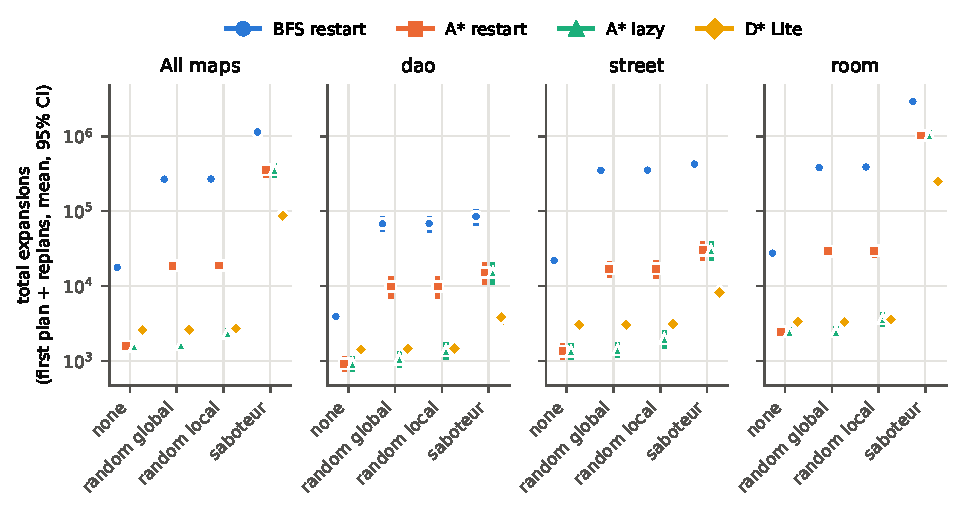
\includegraphics[width=0.8\textwidth]{fig5_total_effort.pdf}
\caption{Total search effort per run (first plan plus all replans), mean with 95\% bootstrap CI,
log scale, for all maps and per map set ($n=360$ runs per point for all maps, 120 per set).}
\label{fig:total}
\end{figure*}

\subsection{Against random changes, lazy A* has the lowest total effort}
Table~\ref{tab:total} and Fig.~\ref{fig:total} show the total effort. Without changes, every
planner only makes its first plan, and \dstar{}'s costs more: 2{,}599 expansions on average
against 1{,}571 for A*, and a median 1.84$\times$ A*'s per problem (interquartile range
1.06--4.95; \dstar{} was cheaper in 80 of 360 problems). Random blocks rarely hit the planned
path (0.5\% of random-global and 4.5\% of random-local blocks did), so lazy A* hardly ever
replans and keeps the lowest mean total effort of all planners (1{,}641 and 2{,}328
expansions). \dstar{} does a little repair work after most blocks but cannot earn back its more
expensive first plan: its total effort is higher than lazy A*'s in 275 (random global) and 243
(random local) of 360 problems (median ratios 1.7 and 1.6, $r=-0.64$ and $-0.37$, both Holm
$p<0.001$; Table~\ref{tab:tests}). Against A* restart, which searches again after every block,
\dstar{}'s total effort is lower (median ratios 0.22 and 0.23, $r=+0.92$ and $+0.91$), and BFS
restart is by far the most expensive planner throughout.

\subsection{Against the saboteur, \dstar{} needs about 4$\times$ fewer expansions}
Every saboteur block lies on the character's path (100\% of saboteur blocks), so lazy A* has
to replan at every event, exactly like A* restart: under the saboteur the two produced identical
runs on all 360 problems. \dstar{}'s mean total effort is 86{,}989 expansions against 354{,}770
for both A* variants, about 4.1$\times$ fewer; it searched less in 305 of the 360 problems
(median ratio 0.36, $r=+0.89$, Holm $p<0.001$). For the replanning effort alone the picture is
the same and even clearer: 84{,}390 against 353{,}199 expansions on average, less in 351 of 360
problems (median ratio 0.27, $r=+0.98$, Holm $p<0.001$; Fig.~\ref{fig:replan}). The direction
holds on every map set (Table~\ref{tab:sets}): the median ratio of total effort is 0.41 on dao,
0.54 on street and 0.29 on room. Across all per-set tests, no map set shows a significant result
in the opposite direction to the overall one; seven comparisons that are significant overall are
not significant in one set (random-global replanning and hitch against A* lazy on dao, the
saboteur hitch on street and room, and random-local total effort against A* lazy on room).

\begin{table}[!t]
\centering
\footnotesize
\setlength{\tabcolsep}{3pt}
\caption{\dstar{} vs.\ A* lazy per map set. Total effort: median \dstar{}/A* lazy ratio (Holm $p$); hitch: W/T/L and Holm $p$. Columns as in Table~\ref{tab:tests}.}
\label{tab:sets}
\begin{tabular}{lccccc}
\toprule
 & & Total, & Total, & \multicolumn{2}{c}{Hitch, saboteur} \\
Set & $n$ & random global & saboteur & W/T/L & $p$ \\
\midrule
Dao & 120 & 1.6 ($<$0.001) & 0.41 ($<$0.001) & 85/0/35 & $<$0.001 \\
Street & 120 & 3.3 ($<$0.001) & 0.54 ($<$0.001) & 67/0/53 & 0.351 \\
Room & 120 & 1.4 ($<$0.001) & 0.29 ($<$0.001) & 61/0/59 & 1.000 \\
\midrule
All & 360 & 1.7 ($<$0.001) & 0.36 ($<$0.001) & 213/0/147 & 0.042 \\
\bottomrule
\end{tabular}
\end{table}


\begin{figure*}[!t]
\centering
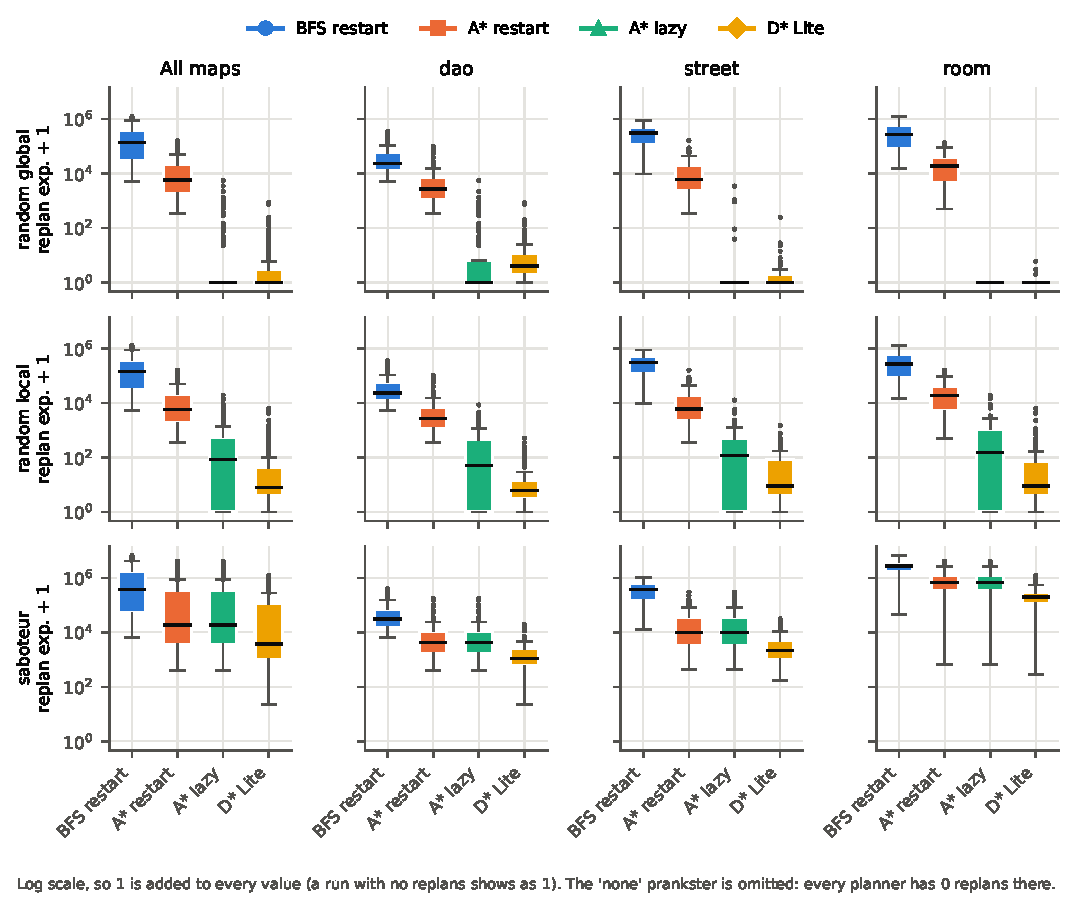
\includegraphics[width=0.8\textwidth]{fig2_replan_boxplot.pdf}
\caption{Replanning effort per run by planner, prankster (rows) and map set (columns). Box:
quartiles; line: median; points: outliers. Log scale, so 1 is added to every value (a run
without replans shows as 1). Without changes every planner has 0 replans (not shown).}
\label{fig:replan}
\end{figure*}

\subsection{The hitch is not reliably reduced}
The worst single replan is shown in Fig.~\ref{fig:hitch} and Table~\ref{tab:tests}. Against the
random pranksters, \dstar{}'s hitches are small and far below A* restart's. Against the
saboteur, however, the evidence is weak. The paired test favours \dstar{} over both A* variants
(213 problems with a smaller hitch, 147 with a larger one; median ratio 0.82, $r=+0.17$, Holm
$p=0.042$), but the effect is small and is not significant on street (Holm $p=0.351$) or room
(61 vs.\ 59 problems, Holm $p=1.000$); only on dao is it clear (85 vs.\ 35, $r=+0.55$). The
typical hitch is smaller (median 1{,}049 against 1{,}697 expansions), but the mean is the same
or slightly larger (20{,}442 against 20{,}388): some \dstar{} repairs are very large. A player
notices exactly these rare, large stalls, so our data do not support the claim that \dstar{}
avoids hitches against a saboteur.

\begin{figure*}[!t]
\centering
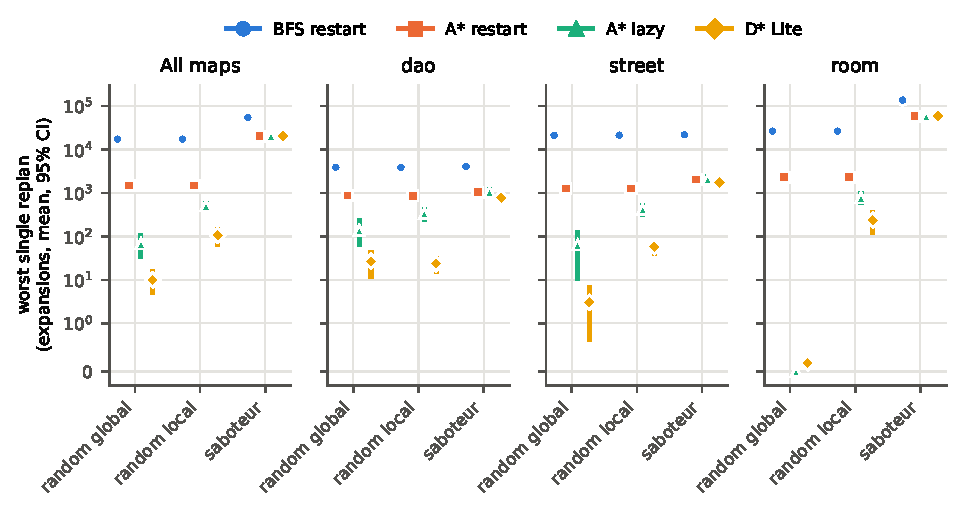
\includegraphics[width=0.9\textwidth]{fig3_hitch.pdf}
\caption{Worst single replan per run (the ``hitch''), mean with 95\% bootstrap CI. Symmetric
log scale (linear below 1), so a mean of exactly 0 (A* lazy on room against random global blocks
never replanned) is still drawn.}
\label{fig:hitch}
\end{figure*}

\subsection{Where the saboteur blocks matters}
Grouping the change events by the distance from the blocked cell to the goal shows that, under
the saboteur, \dstar{}'s advantage depends on that distance.
For blocks within 25 cells of the goal it has no advantage at all (1{,}387 against 1{,}370
expansions per event for A*), while for blocks 100--149 cells from the goal it needs about
7$\times$ fewer (2{,}505 against 18{,}441). This matches the structure of the algorithm: \dstar{}
searches backwards from the goal, so a block near the goal invalidates a large part of its
stored search, while A* restart's cost depends mostly on the distance from the agent to the goal.

\subsection{In Python, \dstar{}'s expansions cost more time}
Table~\ref{tab:time} reports time as a secondary measure. Measured over all runs, an expansion
cost about 54--70\,$\mu$s in \dstar{}, 16--18\,$\mu$s in A* and 3.5--4\,$\mu$s in BFS: each
\dstar{} expansion recomputes $\mathit{rhs}$ for its neighbours and updates the queue, while a BFS
expansion only appends to a list. This 3--4$\times$ difference is far larger than the timing
noise (6--38\%) and it cancels \dstar{}'s advantage in expansions: under the saboteur, \dstar{}
needs about 4$\times$ fewer expansions than A* restart, yet its mean time per run is not lower
(6{,}079 against 5{,}573\,ms). That 9\% difference itself is within the noise, so we do not claim
that \dstar{} is slower, only that its expansion savings do not become time savings in this Python
implementation. The time per run also leaves out \dstar{}'s per-step bookkeeping calls, which did
no expansions but whose time was not logged.

\begin{table*}[!t]
\centering
\footnotesize
\caption{Secondary measure: mean search time per run in ms (first plan + replans), all maps, $n=360$ runs per cell, 95\% bootstrap CI. Not used in any statistical test. Time per expansion over all runs ($\mu$s): BFS restart: 3.8; A* restart: 15.7; A* lazy: 15.6; D* Lite: 68.6.}
\label{tab:time}
\begin{tabular}{lcccc}
\toprule
Planner & None & Random global & Random local & Saboteur \\
\midrule
BFS restart & 65.6 [59.3, 72.4] & 918 [810, 1,033] & 946 [832, 1,059] & 4,429 [3,795, 5,069] \\
A* restart & 28.8 [24.8, 32.9] & 298 [253, 344] & 302 [257, 349] & 5,573 [4,373, 6,814] \\
A* lazy & 27.8 [24.1, 31.8] & 28.7 [24.6, 33.0] & 40.5 [34.6, 47.3] & 5,534 [4,367, 6,737] \\
D* Lite & 140 [128, 153] & 140 [128, 154] & 150 [137, 165] & 6,079 [4,831, 7,449] \\
\bottomrule
\end{tabular}
\end{table*}


\subsection{Path length}
All planners follow optimal routes on the current map, so their paths differ only through the
saboteur's reactions. Without changes and with random changes every planner walks essentially
the optimal length (mean ratio 1.0). Against the saboteur the trips become 2.8--2.9$\times$ longer
on average for every planner, and up to 23.6$\times$ on room
maps, where closing a doorway forces the character around whole rooms.

% =====================================================================================
\section{Application: Outwit}
\label{sec:outwit}
% =====================================================================================

Outwit is a Godot game in which the player is a knight guarding a castle and an AI thief tries to
steal a treasure chest and escape. The knight locks doors (key E) and drops barrel barricades
(key Q) to stop the thief, so in Outwit \emph{the player is the saboteur}: every change the
player makes is chosen to block the thief's route. The thief senses the castle through a
seven-cell field of view, decides between stealing, fighting and fleeing, and follows its plan
with \dstar{}, calling \texttt{move\_start} after every step and \texttt{notify\_changed} with the
cells whose status it has just seen change. The game's own tests show the benefit on its first
level: when a wall drops on the route after four steps, \dstar{} repairs the path with 3
expansions, while a fresh A* search needs 58, and the repaired path has the same length (24
cells) as the fresh one (Table~\ref{tab:port}).

Our results support this design choice, with limits. Measured in expansions, an opponent who
blocks the route on purpose is exactly the case in which \dstar{} needs about four times less
search than both A* variants, and in which lazy A* loses its advantage because every block hits
its path. \dstar{} is therefore the right choice for the thief \emph{in search effort}. Three
differences between the game and our experiment limit this conclusion: the thief does not know
the whole map but senses it, the knight can also unlock doors and the thief can smash barricades
(cells become free again, which our block-only experiment does not test), and GDScript, like
Python, is an interpreted language, so the per-expansion cost that cancelled \dstar{}'s savings in
time in our Python port may matter in the game as well. We did not measure the game's frame
times; a player would also notice the rare large repairs that \dstar{} did not avoid in our data.

% =====================================================================================
\section{Discussion and Threats to Validity}
\label{sec:discussion}
% =====================================================================================

\subsection{Discussion}
The answer depends on what the opponent does. Random changes seldom touch the route, so lazy A*
wins; changes aimed at the route break it every time, so lazy A* degenerates into A* restart and
\dstar{}'s reuse of its earlier search saves about three quarters of the work. This adds a new
axis to the open question of when incremental search
pays~\cite{hernandez2012poorly,hernandez2014mpaa}: whether the changes are aimed at the route.

\subsection{Threats to validity}
\begin{itemize}
\item \textbf{Timing noise.} Python times depend on load, power state and the interpreter;
      identical runs differed by 6--38\%. We draw no conclusion from time alone, and expansions
      do not measure the different cost of an expansion in each algorithm.
\item \textbf{Block-only changes.} Cells are only ever blocked. This is exactly the case in which
      lazy A* is safe; with cells that become free again, the results may differ.
\item \textbf{Full knowledge.} The character learns every change at once; our game's thief senses
      the world through a limited field of view.
\item \textbf{Grid model.} Four directions, unit costs and the Manhattan heuristic; water is treated
      as blocked. The results may not carry over to eight-direction movement or weighted terrain.
\item \textbf{Map selection.} Map sides are at most 256 cells, except for room maps (all
      $512\times512$); 8 maps and 15 problems per set with BFS lengths of 60--250. Because the room
      maps are larger, map set and map size are confounded.
\item \textbf{The saboteur reacts to each planner's own path,} so planners do not face identical
      block sequences, and their trajectories and path lengths differ on the same problem.
\item \textbf{Tie order.} The port reproduces the game's numbers on its level, but that level cannot
      distinguish different orders of cells with exactly equal keys; equality with the game's tie
      order beyond that level is untested.
\item \textbf{A greedy, one-step saboteur.} A stronger interdictor~\cite{israeli2002interdiction}
      might find different, possibly more damaging, blocks.
\end{itemize}

% =====================================================================================
\section{Conclusion}
\label{sec:conclusion}
% =====================================================================================

On 360 problems from real game maps, lazy A* did the least search against random changes, while
against a saboteur \dstar{} needed about four times fewer expansions than both A* variants. Its
worst single replan was not reliably smaller, and in Python its costlier expansions cancelled its
savings in time. For a game in which the player is the saboteur, such as Outwit, \dstar{} is the
better choice in search effort; its repair spikes and per-expansion cost should next be measured
in the game itself, together with partial sensing, opponents that also free cells, and stronger
interdiction models.

\section*{Acknowledgment}
% STUDENT: add or remove as appropriate.
The maps are from the Moving AI Lab benchmarks~\cite{sturtevant2012benchmarks} (Open Data
Commons Attribution License). The code, data and analysis are in our project repository.

\bibliographystyle{IEEEtran}
\bibliography{refs}

\end{document}
